\documentclass[a4paper,12pt]{article}

% Use the Classic Thesis style
%
% \usepackage[nochapters]{classicthesis}

\usepackage[T1]{fontenc}
\usepackage[utf8]{inputenc}

% Use text fonts
%
\usepackage{lmodern}  % the Latin Modern fonts which is an enhanced version of the Computer Modern fonts
% \usepackage{tgschola}  % the Gyre Schola fonts which is an enhanced version of the New Centrury Schoolbook fonts

% Use math fonts
%
% \usepackage{concmath}  % the Concrete Math fonts
% \usepackage{euler}  % the Euler Math fonts
% \usepackage{kerkis}  % the Kerkis fonts

% Some font packages that provide math font may override the text font, the
% following three commands reset it to the default.
%
% For the Latin Modern fonts
%
% \renewcommand{\rmdefault}{lmr}
% \renewcommand{\sfdefault}{lmss}
% \renewcommand{\ttdefault}{lmtt}
%
% For the Gyre Schola fonts
%
% \renewcommand{\rmdefault}{qcs}

\usepackage{amsmath}
\usepackage{amssymb}

% Use the MH bundle
%
% \usepackage{mhsetup}
% \usepackage{mathtools}
% \usepackage{mathstyle}
% \usepackage{breqn}
% \usepackage{empheq}
% \usepackage{flexisym}

% Use AMS-style theorem
%
\usepackage{amsthm}
% \theoremstyle{definition}
% \newtheorem{theorem}{Theorem}

% Use MATH formulas in PARagraph mode Typesetting Inference Rules
% 
\usepackage{mathpartir}

\usepackage{tikz}
\usepackage{tikz-qtree}
\usepackage{bigfoot}

% New commands
%
\newcommand{\term}[1]{\textsf{#1}}
\newcommand{\appl}[2]{#1\inparens{#2}}
\newcommand{\eval}[2]{#1 \Longrightarrow #2}
\newcommand{\redc}[2]{#1 \longrightarrow #2}

\usepackage{stmaryrd}  % the St Mary’s Road symbol font


\newcommand{\atangles}[1]{\langle#1\rangle}
\newcommand{\atparens}[1]{(#1)}
\newcommand{\atbracks}[1]{[#1]}
\newcommand{\atbraces}[1]{\{#1\}}
\newcommand{\atfloors}[1]{\lfloor#1\rfloor}
\newcommand{\atceils}[1]{\lceil#1\rceil}
\newcommand{\atucorners}[1]{\ulcorner#1\urcorner}
\newcommand{\atlcorners}[1]{\llcorner#1\lrcorner}
\newcommand{\atlparens}[1]{\llparenthesis#1\rrparenthesis}
\newcommand{\atlbracks}[1]{\llbracket#1\rrbracket}
\newcommand{\atbars}[1]{|#1|}
\newcommand{\atbbars}[1]{\|#1\|}

\newcommand{\inangles}[1]{\langle#1\rangle}
\newcommand{\inparens}[1]{\left(#1\right)}
\newcommand{\inbracks}[1]{\left[#1\right]}
\newcommand{\inbraces}[1]{\left\{#1\right\}}
\newcommand{\infloors}[1]{\left\lfloor#1\right\rfloor}
\newcommand{\inceils}[1]{\left\lceil#1\right\rceil}
\newcommand{\inucorners}[1]{\left\ulcorner#1\right\urcorner}
\newcommand{\inlcorners}[1]{\left\llcorner#1\right\lrcorner}
\newcommand{\inlparens}[1]{\left\llparenthesis#1\right\rrparenthesis}
\newcommand{\inlbracks}[1]{\left\llbracket#1\right\rrbracket}
\newcommand{\inbars}[1]{\left|#1\left|}
\newcommand{\inbbars}[1]{\left\|#1\right\|}

\newcommand{\texterr}[1]{\textcolor{red}{#1}}

\newenvironment{grammar}
 {\begin{center}\small\begin{tabular}{rrclr}}
 {\end{tabular}\normalsize\end{center}}
\newcommand{\prodhead}[5]{#1 & #2 & #3 & #4 & #5 \\}
\newcommand{\prodrule}[3]{      & & #1 & #2 & #3 \\}



% Front elements
%
\title{
 Programming Languages and Types \\~\\
 \textbf{Exercise 10}
}
\author{
 Yi Dai
}

\begin{document}

\maketitle

\section{Abstract Syntax vs. Concrete Syntax}

Presented below is the syntax of a language (call it AE) for (a subset of) arithmetic
expressions.
\begin{gather*}
 e \in Exp \\
 n \in Nat \\
 o \in Opr
\end{gather*}
\begin{grammar}
 \prodhead{(expression)}{$e$}{::=}{$n$}{(numeral)}
 \prodrule{|}{$e_1\ o\ e_2$}{(compound)}
 \\
 \prodhead{(operator)}{$o$}{::=}{\tt +}{(plus)}
 \prodrule{|}{\tt -}{(minus)}
 \prodrule{|}{\tt *}{(times)}
 \prodrule{|}{\tt /}{(divides)}
\end{grammar}
In theoretical formulation, such a presentation is usually \emph{said} to define
the \term{abstract syntax} of a language for the following reasons: first, it
captures all the structures of the language; second, the grammar is not concerned
to handle ambiguity but leaves the deal to convention (like operator precedence,
associativity and parentheses).  However, the syntax thus defined is only
\emph{semi-abstract}.  It is \emph{not fully abstract} since it uses \term{infix
notation}.  It is \emph{not completely concrete} either, since it does not handle
the ambiguity of infix notation.  A fully abstract syntax (with the declaration of
syntactic categories and the definition of operators omitted just for conciseness)
for AE could be:
\begin{grammar}
 \prodhead{(expression)}{$e$}{::=}{$\appl{num}{n}$}{(numeral)}
 \prodrule{|}{$\appl{com}{o, e_1, e_2}$}{(compound)}
\end{grammar}
It describes the leaf and node structure that build up syntax trees
\begin{center}
 \begin{tabular}{c c}
  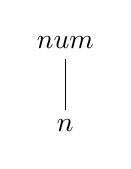
\begin{tikzpicture}
   \Tree [ .$num$ $n$ ]
  \end{tikzpicture}
  &
  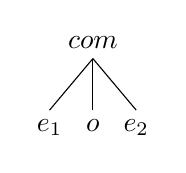
\begin{tikzpicture}
   \Tree [ .$com$ $e_1$ $o$ $e_2$ ]
  \end{tikzpicture}
 \end{tabular}
\end{center}
and can be readily implemented using tree-like data structures, for example, in
Scala as:
\begin{verbatim}
sealed abstract class Exp
type Opr = String
type Nat = Int
case class Num(nat : Nat) extends Exp
case class Com(opr : Opr, lhs : Exp, rhs : Exp) extends Exp
\end{verbatim}
It also gives us the freedom to choose the concrete syntax for the language, say
\term{prefix} or \term{postfix notation} instead of infix notation.  Usually infix
notation is chosen for its readability.  Thus semi-abstract syntax given above is
widely spread.

\section{Inductive Definitions and Rule Induction}

\subsection{Inductive Definitions}

\begin{enumerate}
 \item Inductively-defined sets: natural numbers, arithmetic expressions, etc.
  \begin{mathpar}
   \inferrule
    {n \in Nat}
    {n \in Exp}\ \textsc{Num} \qquad
   \inferrule
    {e_1 \in Exp \and e_2 \in Exp \and o \in Opr}
    {e_1\ o\ e_2 \in Exp}\ \textsc{Com}
  \end{mathpar}

 \item Inductively-defined relations: $m\ Div\ n$, evaluation relation of
  arithmetic expressions, etc.
  \begin{mathpar}
   \inferrule
    { }
    {m\ Div\ 0}\ \textsc{DNil} \qquad
   \inferrule
    {m\ Div\ n}
    {m\ Div\ n + m}\ \textsc{DSum}
  \end{mathpar}
\end{enumerate}

\noindent
Note that a relation is just a set of tuples.  Hence $m\ Div\ n$ is essentially an
inductively-defined set of pairs $\inparens{m, n}$.

\subsection{Rule Induction}

Rule induction rules!  For every \emph{sound} inductive definition, we have a
\term{rule induction} principle for free.  The notion is simple, to prove some
property $P$ for every element of an inductively defined set, it is sufficient to
prove $P$ holds for the conclusion assuming $P$ holds for all the premises, for
every rule in the inductive definition.  That is, for every rule of the form

\begin{mathpar}
 \inferrule
  {premise_1 \and \ldots \and premise_n}
  {conclusion},
\end{mathpar}

\noindent
prove $\appl{P}{conclusion}$ assuming $\appl{P}{premise_1}$, $\ldots$,
$\appl{P}{premise_n}$, for every $n \in \mathbf{N}$.  When $n = 0$, a rule becomes
an axiom.  In this case, you have to prove $P(conclusion)$ ``out of thin air''.

\begin{enumerate}
 \item Prove that the sum of the first $n$ natural numbers is
  $\frac{n\inparens{n + 1}}{2}$, that is, prove
  \[ \sum_{i = 0}^{n} i = \frac{n\inparens{n + 1}}{2} \]
 \item Prove that $m\ Div\ n_1$ and $m\ Div\ n_2$ implies $m\ Div\ (n_1 + n_2)$.
  \begin{proof}
   We prove the property
   \[
     \appl{P}{m\ Div\ n_1} = \inbracks{\forall n_2 \in \mathbf{N}, m\ Div\ n_2\
     \text{implies}\ m\ Div\ (n_1 + n_2)}
   \]
   for every $m\ Div\ n_1$ by rule induction on $m\ Div\ n_1$.

   \begin{itemize}
    \item Base case: for $\inferrule{ }{m\ Div\ 0}$, we want to prove
     \[
       \appl{P}{m\ Div\ 0} = \inbracks{\forall n_2 \in \mathbf{N}, m\ Div\ n_2\
       \text{implies}\ m\ Div\ (0 + n_2)}
     \]

     Since $0 + n_2 = n_2$, the goal is to prove $m\ Div\ n_2$ implies $m\ Div\ n_2$,
     which is trivial.
    \item Inductive case: for $\inferrule{m\ Div\ n_1}{m\ Div\ n_1 + m}$, we want to
     prove
     \begin{multline*}
      \appl{P}{m\ Div\ \inparens{n_1 + m}} = \\ \inbracks{\forall n_2 \in \mathbf{N},
       m\ Div\ n_2\ \text{implies}\ m\ Div\ (n_1 + m + n_2)},
     \end{multline*}
     assuming the inductive hypothesis
     \begin{multline*}
      \appl{P}{m\ Div\ n_1} = \\ \inbracks{\forall n_2 \in \mathbf{N}, m\ Div\ n_2\
      \text{implies}\ m\ Div\ (n_1 + m)},
     \end{multline*}

     Suppose $\forall n_2 \in \mathbf{N}, m\ Div\ n_2$, by the inductive hypothesis,
     we have $m\ Div\ \inparens{n_1 + n_2}$, then apply the rule \textsc{DSum} by
     instantiating $n$ with $\inparens{n_1 + n_2 + m}$, we can conclude $m\ Div\
     \inparens{m\ Div\ n_1 + n_2 + m}$, that is,
     \begin{mathpar}
      $\inferrule{m\ Div\ \inparens{n_1 + n_2}}{m\ Div\ \inparens{n_1 + n_2 + m}}\
       \textsc{DSum}.
     \end{mathpar}
     Further, from $m\ Div\ \inparens{n_1 + n_2 + m}$, by associativity and commutativity 
     of $+$, we can derive $m\ Div\ \inparens{n_1 + m + n_2}$, which is exactly what we 
     want to prove.
   \end{itemize}
   Therefore, we have proved $\appl{P}{m\ Div\ n_1}$ for every $m\ Div\ n_1$, that is,
   $\forall m, n_1, n_2 \in \mathbf{N}, m\ Div\ n_1$ and $m\ Div\ n_2$ implies $m\ Div\
   (n_1 + n_2)$.
  \end{proof}
\end{enumerate}

\section{Evaluation Semantics vs. Reduction Semantics}

\begin{enumerate}
 \item Give the \term{(structural) evaluation semantics} (aka. \term{(structural)
  big-step (operational) semantics}, \term{natural semantics}) for AE.

  We first define a syntactic category for values.  For convenience, we integrate
  it into the semi-abstract syntax given above for AE.  Hereby we have the following
  syntax definition:
  \begin{gather*}
   e \in Exp \\
   n \in Int \\
   o \in Opr \\
   v \in Val
  \end{gather*}

  \begin{grammar}
   \prodhead{(expression)}{$e$}{::=}{$v$}{(value)}
   \prodrule{|}{$e_1\ o\ e_2$}{(compound)}
   \\
   \prodhead{(operator)}{$o$}{::=}{\tt +}{(plus)}
   \prodrule{|}{\tt -}{(minus)}
   \prodrule{|}{\tt *}{(times)}
   \prodrule{|}{\tt /}{(divides)}
   \\
   \prodhead{(value)}{$v$}{::=}{$n$}{(numeral)}
  \end{grammar}
  
  The evaluation semantics for arithmetic expressions is given by a evaluation relation
  between expressions and values (the final form of expressions after a series of
  reductions), notated as $\eval{e}{v}$, inductively defined as follows:
  \begin{mathpar}
   \inferrule
    { }
    {\eval{v}{v}}\ \textsc{EvV} \qquad
   \inferrule
    {\eval{e_1}{v_1} \and \eval{e_2}{v_2}}
    {\eval{e_1\ o\ e_2}
          {\inucorners{\appl{op}{\inlcorners{o}, \inlcorners{v_1}, \inlcorners{v_2}}}}}
    \ \textsc{EvC}
  \end{mathpar}
  The inductive definition contains two rules, one axiom named \textsc{EvV}, one named
  \textsc{EvC} with two premises. The axiom \textsc{EvV} essentially says that a value
  evaluates to itself. In this example, a value can only be a numeral. The rule
  \textsc{EvC} says, to obtain the value of a compound expression $e_1\ o\ e_2$, evaluate
  $e_1$ to $v_1$ and $e_2$ to $v_2$, then use a mathematical function (in the meta-language)
  $op$ which applies the mathematical operation corresponding to $o$ to the numbers
  corresponding to $v_1$ and $v_2$ to get the result number, and finally obtain the numeral
  in the object-language (AE) of the number in the meta-language (mathematics and English).
  The notation $\inucorners{\ }$ goes from the meta-level to the object-level, whereas the
  notation $\inlcorners{\ }$ goes the other way around.  For example, $\inucorners{1} =
  \texttt{1}$ and $\inlcorners{\texttt{1}} = 1$.  \verb|1| is a \emph{numeral} in the
  object-language, while $1$ is a \emph{number} in the meta-language.

  These rules should remind you of the interpreter you have crafted for arithmetic
  expressions.

  Here is a demonstration of how to apply these evaluation rules to obtain the value of
  an example expression: \verb|1 + 2 * 3 - 4|. Note that we assume the meta-function $op$
  can handle the operators \verb|+|, \verb|*| and \verb|-| correctly.
  {\footnotesize
  \begin{mathpar}
   \inferrule
    {\inferrule
      {\inferrule
        { }
        {\eval{\texttt{1}}{\texttt{1}}}
       \ \textsc{EvV}
       \and
       \inferrule
        {\inferrule
          { }
          {\eval{\texttt{2}}{\texttt{2}}}
         \ \textsc{EvV}
         \and
         \inferrule
          { }
          {\eval{\texttt{3}}{\texttt{3}}}
         \ \textsc{EvV} }
        {\eval
          {\texttt{2 * 3}}
          {\inucorners{
            \appl{op}{\inlcorners{\texttt{*}}, \inlcorners{\texttt{2}}, \inlcorners{\texttt{3}}}
           } = \texttt{6} } }
       \ \textsc{EvC} }
      {\eval
        {\texttt{1 + 2 * 3}}
        {\inucorners{
          \appl{op}{\inlcorners{\texttt{+}}, \inlcorners{\texttt{1}}, \inlcorners{\texttt{6}}}
         } = \texttt{7} } }
     \ \textsc{EvC}
     \and
     \inferrule
      { }
      {\eval{\texttt{4}}{\texttt{4}}}
     \ \textsc{EvV} }
    {\eval
      {\texttt{1 + 2 * 3 - 4}}
      {\inucorners{
        \appl{op}{\inlcorners{\texttt{-}}, \inlcorners{\texttt{7}}, \inlcorners{\texttt{4}}
       } } = \texttt{3} } }
   \ \textsc{EvC}
  \end{mathpar} }
  So we know the value of the expression \verb|1 + 2 * 3| is \verb|7|.
  
  As an exercise, try to derive the evaluation of the expression \verb|1 * 2 + 3 * 4| using the
  above rules.

 \item Compare evaluation semantics and \term{(structural) reduction semantics} (aka.
  \term{(structural) small-step (operational) semantics}).

  The reduction semantics for arithmetic expressions is given by a reduction relation
  between expressions, notated as $\redc{e}{e'}$, inductively defined as follows:
  \begin{mathpar}
   \inferrule
    { }
    {\redc{v_1\ o\ v_2}
          {\inucorners{\appl{op}{\inlcorners{o}, \inlcorners{v_1}, \inlcorners{v_2}}}} }
   \ \textsc{Red} \\
   \inferrule
    {\redc{e_1}{e_1'}}
    {\redc{e_1\ o\ e_2}{e_1'\ o\ e_2}}
   \ \textsc{RdL}
   \qquad
   \inferrule
    {\redc{e_2}{e_2'}}
    {\redc{e_1\ o\ e_2}{e_1\ o\ e_2'}}
   \ \textsc{RdR}
  \end{mathpar}
  The axiom \textsc{Red} says that we can invoke the primitve operation corresponding to
  the operator $o$ only when both its operands have reduced to values. The rule \textsc{RdL}
  covers one-step reduction of the left operand of a compound expression, while the rule
  \textsc{RdR} covers that of the right operand. Note that there is no longer a rule like
  $\redc{v}{v}$, since a value cannot be reduced in one step to anything. If such a
  rule is included in the definition, after an expression is reduced to a value, one can
  keep reducing it to itself by applying this rule till the end of the world (Who knows
  when it is, maybe Maya people?).

  Here is a demonstration of how to apply these reduction rules to obtain the final result
  the same expression \verb|1 + 2 * 3 - 4|. Again, we assume the correctness of the
  meta-function $op$.
  \begin{mathpar}
   \inferrule
    {\inferrule
      {\inferrule
        { }
        {\redc
          {\texttt{2 * 3}}
          {\inucorners{
            \appl{op}{\inlcorners{\texttt{*}}, \inlcorners{\texttt{2}}, \inlcorners{\texttt{3}}}
           } = \texttt{6} } }
       \ \textsc{Red} }
      {\redc{\texttt{1 + 2 * 3}}{\texttt{1 + 6} } }
     \ \textsc{RdR} }
    {\redc{\texttt{1 + 2 * 3 - 4}}{\texttt{1 + 6 - 4}}}\ \textsc{RdL}
  \end{mathpar}
  This is just one-step reduction. To reach the final result of the expression, we need
  continue reducing the result expression \verb|1 + 6 - 4|:
  \begin{mathpar}
   \inferrule
    {\inferrule
      { }
      {\redc
        {\texttt{1 + 6}}
        {\inucorners{
          \appl{op}{\inlcorners{\texttt{+}}, \inlcorners{\texttt{1}}, \inlcorners{\texttt{6}}}
         } = \texttt{7} } }
     \ \textsc{Red} }
    {\redc{\texttt{1 + 6 - 4}}{\texttt{7 - 4}}}\ \textsc{RdL}
  \end{mathpar}
  Go on reducing \verb|7 - 4|:
  \begin{mathpar}
   \inferrule
    { }
    {\redc
      {\texttt{7 - 4}}
      {\inucorners{
        \appl{op}{\inlcorners{\texttt{-}}, \inlcorners{\texttt{7}}, \inlcorners{\texttt{4}}}
       } = \texttt{3} } }
   \ \textsc{Red}
  \end{mathpar}
  Now that the numeral \verb|3| can no longer be reduced, it is the result of the whole
  expression. So we have seen that the original expression \verb|1 + 2 * 3 - 4| is reduced
  by \emph{three} steps to the numeral \verb|3|, that is,
  \[
    \redc{\texttt{1 + 2 * 3 - 4}}{\redc{\texttt{1 + 6 - 4}}{\redc{\texttt{7 - 4}}{\texttt{3}}}}
  \]
  Note that the number of reduction steps is clearly indicated by the number of occurrences
  of the rule \textsc{Red} in the three derivation trees.
  
  As an exercise, try to derive the multi-step reduction of the expression \verb|1 * 2 + 3 * 4|
  using the above rules.
\end{enumerate}

\end{document}
